\documentclass[conference]{IEEEtran}

% ==================== PACKAGES ====================
\usepackage{cite}
\usepackage{amsmath,amssymb,amsfonts}
\usepackage{graphicx}
\graphicspath{{./}}
\usepackage{textcomp}
\usepackage{xcolor}
\usepackage{booktabs}
\usepackage{listings}
\usepackage{hyperref}
\usepackage{float}
\usepackage{enumitem}
\usepackage{multirow}
\usepackage{array}

% ==================== LISTINGS STYLE ====================
\lstset{
  basicstyle=\ttfamily\footnotesize,
  breaklines=true,
  frame=single,
  language=Python,
  keywordstyle=\color{blue},
  commentstyle=\color{gray},
  stringstyle=\color{red},
  showstringspaces=false
}

\begin{document}

% ==================== TITLE ====================
\title{LLM-Based Automatic Unit Test Generation Using Focal-Method Datasets}

\author{
\small
\begin{tabular*}{\textwidth}{@{\extracolsep{\fill}}cccc@{}}
\begin{tabular}{@{}c@{}}
\textbf{Siwani Sah} \\
\scriptsize
\textit{Department of Computer Science} \\
\textit{Florida Polytechnic University} \\
Lakeland, Florida, USA \\
ssah2942@floridapoly.edu
\end{tabular}
&
\begin{tabular}{@{}c@{}}
\textbf{Saarupya Sunkara} \\
\scriptsize
\textit{Department of Computer Science} \\
\textit{Florida Polytechnic University} \\
Lakeland, Florida, USA \\
vsunkara3613@floridapoly.edu
\end{tabular}
&
\begin{tabular}{@{}c@{}}
\textbf{Alexandra Hyatali} \\
\scriptsize
\textit{Department of Computer Science} \\
\textit{Florida Polytechnic University} \\
Lakeland, Florida, USA \\
ahyatali@floridapoly.edu
\end{tabular}
\end{tabular*}
}

\maketitle

% ==================== ABSTRACT ====================
\begin{abstract}
 In this paper, we examine whether a large language model can take some of the burden of writing unit tests by hand. This is one of the most time consuming parts of software development, so we are trying to solve this by automatically generating pytest-style unit tests for Python functions. The end-to-end pipeline we built pulls real-world functions from the pyMethods2Test dataset and feeds them to the Llama~3 model through Ollama, which generates a total of 300 tests. This then evaluates whatever the model produces. To examine how prompt design affects results three different prompting strategies were used. These were a simple baseline, a context-enriched prompt, and a fully structured advanced prompt. We then compared the tests that each of these generated. The advanced prompt led to an average of 9.38 assertions per test and edge-case coverage across every sample based on keyword detection. The experiment also made the current limits of LLM-generated code hard to disregard. The results showed 53\% of the generated tests were syntactically valid Python, and 47\%  contained syntax errors. These findings suggest that large language models are a genuinely useful starting point for test generation, but they are not yet a replacement for human review and post-processing.
\end{abstract}

\begin{IEEEkeywords}
Large Language Models, Unit Test Generation, Prompt Engineering, Software Testing, Llama~3, Automated Testing
\end{IEEEkeywords}

% ==================== 1. INTRODUCTION ====================
\section{Introduction}

Unit testing is widely recognized as a cornerstone of reliable software, yet in practice it is one of the first things developers often reduce when deadlines are tight. Writing thorough tests requires more than just the expected behavior through a function. It needs understanding along with the edge cases, how things can go wrong and the boundary values. This process takes time and in real world projects the test suite ends up thinner than anyone would like.

 An interesting possibility that Large Language Models (LLMs) have presented is what if a model could draft those tests automatically? Review of the outputs and corrections would still need to be completed, but a rough first draft could save a significant amount of effort. Before this idea can be reliably used in practice, we need to understand the quality and limitations of the tests generated by current models.

We conducted an experiment to better evaluate this. We built a pipeline that takes real Python functions from the pyMethods2Test dataset \cite{tufano2022methods2test}, sends them to Llama~3 (a state-of-the-art open-source LLM) running locally through Ollama, and collects the pytest test cases the model generates in response. We then evaluate the generated tests along several dimensions. We look at how many assertions they contain, whether the code is syntactically valid, what kind of issues appear when it is not, and whether they cover edge cases. 

To examine the impact of prompt phrasing, we experimented with three progressively more detailed prompting strategies. The simplest prompt asks for tests given a function name. The most detailed one provides the function body, specifies the kinds of edge cases to include, asks for parameterized tests, and tells the model to output only valid Python.

Our main contributions are as follows:

\begin{itemize}[leftmargin=*]
    \item We design and implement an end-to-end pipeline for LLM-based unit test generation that goes from a raw dataset to evaluated results with an interactive dashboard.
    \item We compare three prompting strategies and show how structured, detailed prompts improve test quality.
    \item We provide a detailed failure analysis that categorizes how LLM-generated tests are limited. This shows practical guidance for anyone looking to use this approach in a real project.
\end{itemize}

% ==================== 2. BACKGROUND & RELATED WORK ====================
\section{Background and Related Work}

\subsection{Automated Test Generation}

Automatic test generation has been studied for several years. Traditional tools like Randoop \cite{pacheco2007randoop} produce tests by generating random sequences of method calls and checking whether any of them trigger an exception. EvoSuite \cite{fraser2011evosuite} takes a more guided approach, using evolutionary algorithms to generate JUnit tests that maximize code coverage. These tools are effective for certain kinds of code, but they often produce tests that are harder for humans to interpret. They rarely capture the intent behind the code the way a developer-written test would.

\subsection{LLMs for Code Generation}

Large language models have changed the way code can be generated significantly. Models like Codex \cite{chen2021codex}, which powers GitHub Copilot, were trained on enormous bodies of source code and can generate functional code, classes, and tests when given a natural-language description. More recent open-source models Llama~2, Llama~3 \cite{touvron2023llama}, CodeLlama, and StarCoder \cite{li2023starcoder} have made these capabilities available in places where data cannot be sent to a cloud API. Being able to run a model locally, as we do in this project through Ollama, is especially important in enterprise environments with strict data-privacy requirements.

\subsection{Prompt Engineering}

One of the most effective ways to improve LLM output is using prompt engineering. We see through research that the way the task is framed can produce different results on the same model. Some types of prompt engineering are few-shot prompting, chain-of-thought prompting \cite{wei2022chain}, and role-based prompting (telling the model to act as a specific kind of expert) which have been shown to improve performance in code-related tasks. In this project, we use structured instructions and role-based prompting to push the model toward better test generation.

\subsection{Focal-Method Datasets}

The pyMethods2Test dataset \cite{tufano2022methods2test} pairs Python functions with the unit tests that developers actually wrote for them. Each record identifies a `focal method,' which is the function under test along with its file location and line range. This type of dataset is useful because it provides a ground truth for comparison. We can compare what the model generated to see whether it captures the same concerns a human tester addressed. This allows the dataset to become particularly suitable for evaluating the quality of LLM-generated tests.

\subsection{Positioning of This Work}

Most prior work on LLM-based test generation have focused on closed-source models and evaluated output through code-coverage metrics. Our work focuses on several key differences. First, we use an open-source model (Llama~3) running locally, which allows the system to be reproducible without requiring API access. Second, we evaluate not only coverage but also elements such as extra text in the generated output and syntactic validity. Third, we compare multiple prompting strategies on the same set of methods, which provides a better understanding of how much prompt design affects results.

% ==================== 3. DESIGN / METHODOLOGY ====================
\section{Design and Methodology}

\subsection{System Architecture}

Our system is designed as a modular pipeline with six stages. Each stage is implemented as a standalone Python script. This structure makes it easier to replace or modify components, change the evaluation criteria, or rerun a single stage without going back to the beginning.

The pipeline proceeds as follows:

\begin{enumerate}[leftmargin=*]
    \item \textbf{Method Extraction} (\texttt{extract\_methods.py}): Walks through every JSON file in the pyMethods2Test dataset and extracts the metadata for each focal method, including the source file path, method name, and line range.
    \item \textbf{Sampling} (\texttt{sample\_methods.py}): Randomly selects a fixed number of methods from the full extracted set to keep the experiment manageable.
    \item \textbf{Test Generation} (\texttt{generate\_tests\_llm.py} and \texttt{generate\_tests\_llm\_advanced.py}): Sends each sampled method to Llama~3 via the Ollama Python client and records the generated output.
    \item \textbf{Evaluation} (\texttt{evaluate\_tests.py}): Counts assertions using regular expressions and checks for edge-case keywords in the generated output.
    \item \textbf{Failure Analysis} (\texttt{failure\_analysis.py}): Compiles each generated test with Python's built-in \texttt{compile()} function, flags tests that contain no assertions, and detects conversational text that the model included alongside the code.
    \item \textbf{Dashboard} (\texttt{dashboard.py}): Presents all results through a Streamlit web application with live metrics, charts, and an interactive test explorer.
\end{enumerate}

\subsection{Dataset Description}

We used the pyMethods2Test dataset, which is a large-scale collection of Python methods paired with their corresponding developer-written test cases. The dataset is organized as a set of JSON files that maps test files to focal methods. After extraction, our pipeline identified a pool of methods drawn from well-known open-source projects, including OpenStack Cinder, Keras, NumPy, Ansible, and Docker Compose. We generated multiple tests per focal method, which resulted in a total of 300 generated tests. Through this the experiment is manageable and allows for a controlled comparison of prompting strategies. The pipeline is designed to scale to larger samples without requiring code changes.

\begin{figure}[htbp]
\centerline{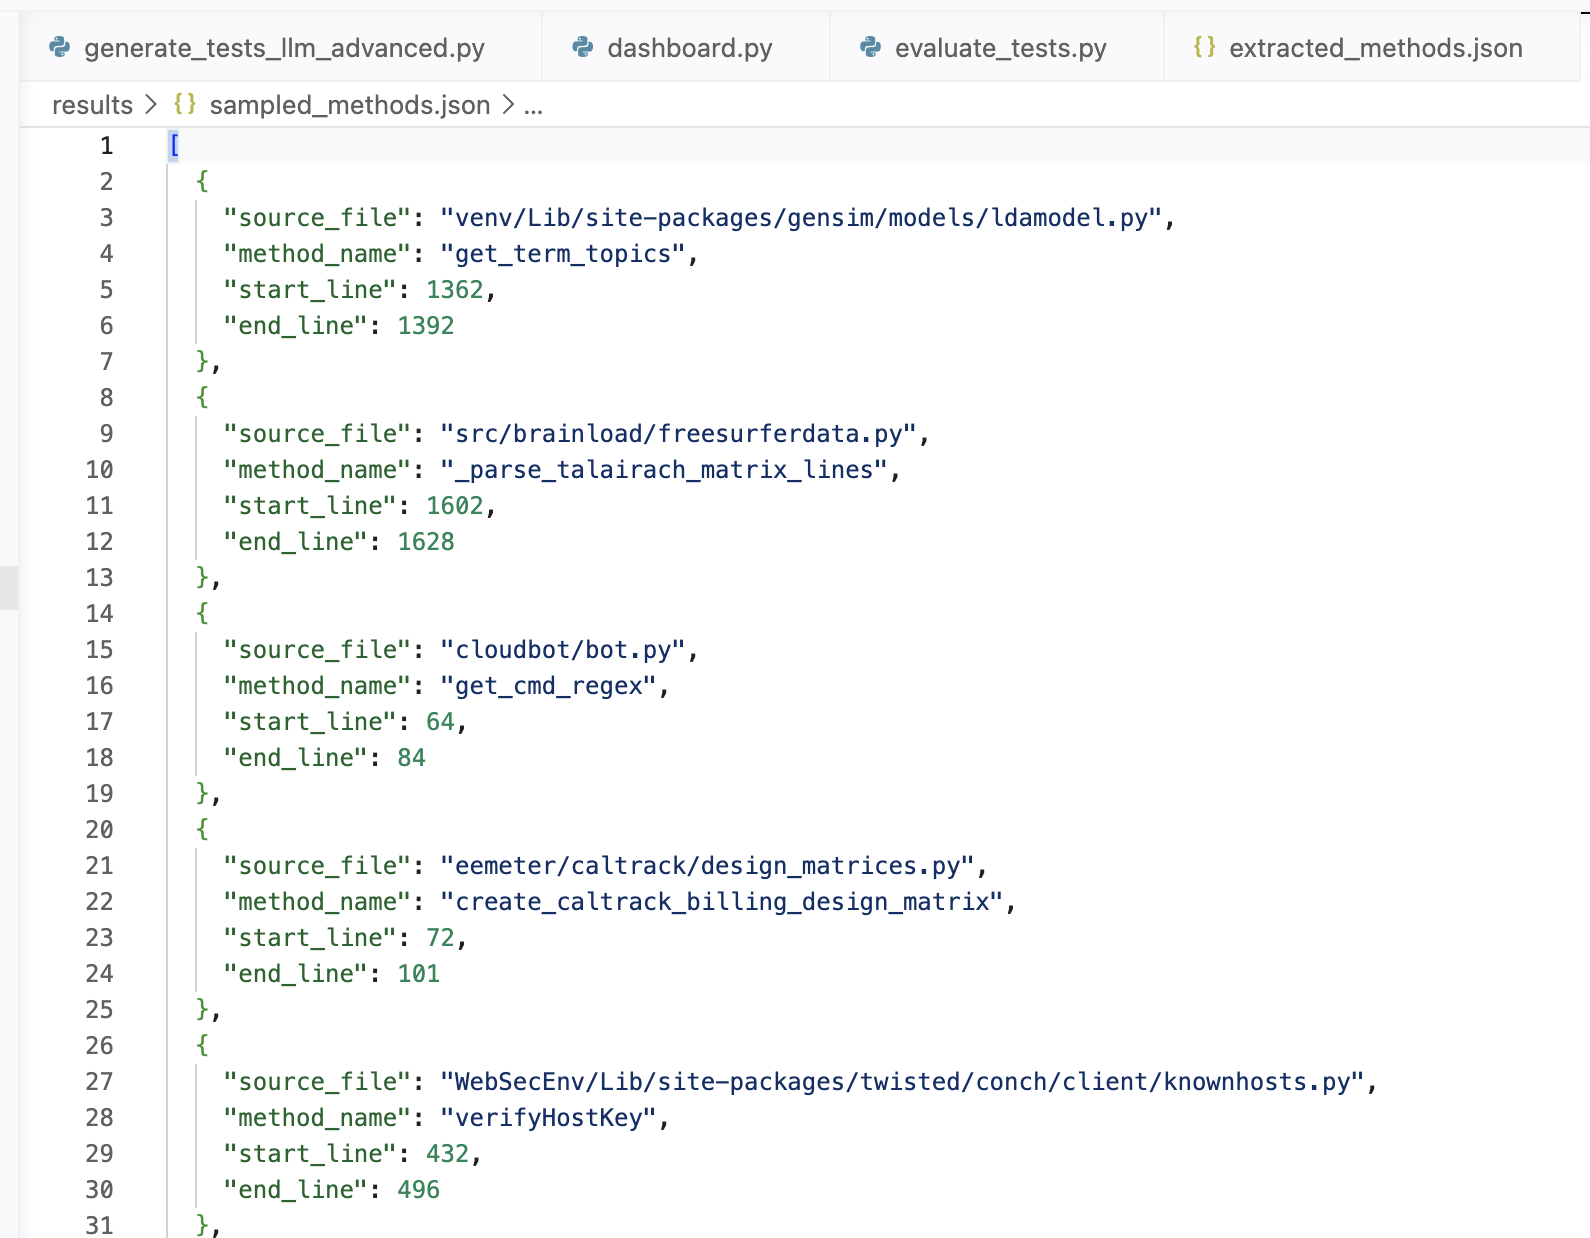
\includegraphics[width=0.80\linewidth]{Images/extracted_methods1.png}}
\caption{Sample of extracted focal methods from the pyMethods2Test dataset}
\label{fig:extracted_methods}
\end{figure}

\subsection{Prompting Strategies}

We designed three prompting strategies, each building on the previous one:

\subsubsection{Baseline Prompt}
The prompt provides the model with the function name and basic instructions to generate pytest unit tests:

\begin{lstlisting}
Generate pytest unit tests for a Python
function named '{method_name}'.

Requirements:
- Include normal cases
- Include edge cases
- Include assertions
\end{lstlisting}

\subsubsection{Context-Enriched Prompt}
This prompt introduces a role assignment and adds more specific structural guidance and expected behavior:

\begin{lstlisting}
You are a professional Python developer.

Write pytest unit tests for the function
'{method_name}'.

The tests should:
- Follow pytest format
- Include multiple assertions
- Include edge cases
- Include boundary conditions
- Simulate realistic developer-written tests
\end{lstlisting}

\subsubsection{Advanced Prompt}
This prompt includes the full function body when available, lists the specific edge-case categories the model should cover, asks for parameterized tests, and enforces strict formatting rules to improve output quality:

\begin{lstlisting}
You are a professional Python developer.

Here is the function:
{method_code}

Generate pytest unit tests.

Requirements:
- Include normal test cases
- Include edge cases:
  - zero values
  - negative values
  - empty inputs
  - invalid inputs
  - boundary conditions
  - large inputs
- Also include these specific edge cases:
  {edge_cases}
- Use multiple assertions
- Use pytest.mark.parametrize where possible
- Create multiple test functions

STRICT RULES:
- Output only valid Python pytest code
- Do not include explanations outside code
- Add explanation only as comments inside tests
- Each test function must include at least
  2 assertions
\end{lstlisting}

\subsection{Edge-Case Generation Heuristic}

For the advanced prompt, we developed a simple heuristic that analyzes the function name and suggests relevant edge cases. For example, if the function name contains `add' or `sum,' the heuristic suggests inputs like \texttt{(0,0)}, \texttt{(-1,-2)}, and \texttt{(1000000,1000000)}. If it contains `divide,' the suggestions include a division-by-zero case. Functions involving lists get empty-list and singleton-list cases. This approach is intentionally simple because a more advanced system would use static analysis but it shows that simple heuristics can improve generated tests relevance. 

\subsection{LLM Configuration}

We used the Llama~3 model through Ollama framework, an open-source tool for running LLMs locally. We used the default model parameters (temperature, top-$p$, etc.) provided by Ollama to ensure reproducibility. Each method was processed independently in a single-turn conversation with no prior context carried over between methods.

% ==================== 4. EVALUATION ====================
\section{Evaluation}

\subsection{Experimental Setup}

We ran the full pipeline on a set of randomly sampled focal methods drawn from the pyMethods2Test dataset. Each method was processed through all three prompting strategies sequentially. The failure analysis and evaluation scripts were then applied to the output of the advanced prompt. This was done because that strategy produced the most detailed tests providing the most interesting data to analyze.

\subsection{Metrics}

We measured five quantities:

\begin{itemize}[leftmargin=*]
    \item \textbf{Total Assertions}: The number of \texttt{assert} statements found across all generated tests, counted using regular expressions.
    \item \textbf{Average Assertions per Test}: The mean number of assertions per generated test case.
    \item \textbf{Edge-Case Coverage}: The proportion of generated tests that contain at least one keyword associated with edge cases (such as \texttt{None}, \texttt{0}, \texttt{negative}, \texttt{[]}, \texttt{-1}, or \texttt{large}).
    \item \textbf{Syntactic Validity}: The proportion of generated tests that compile successfully under Python's \texttt{compile()} function (syntactic validity) after cleaning.
    \item \textbf{Extra Text Rate}: The proportion of generated tests that include conversational text (e.g., ``Here are the pytest\ldots'') that would need to be removed before execution.
\end{itemize}

\subsection{Baselines}

Since our primary goal is to compare prompting strategies, we want the baseline prompt to serve as our experimental baseline. Our results are compared qualitatively against results reported in prior work on ChatGPT and Codex-based test generation.

\subsection{Results}

Advanced prompting strategy results are summarized below.


Table~\ref{tab:eval_results} summarizes the evaluation results for the advanced prompting strategy.

\begin{table}[H]
\centering
\caption{Evaluation Results Advanced Prompt}
\label{tab:eval_results}
\begin{tabular}{lc}
\toprule
\textbf{Metric} & \textbf{Value} \\
\midrule
Total Generated Tests & 300 \\
Total Assertions & 2814 \\
Average Assertions per Test & 9.38 \\
Edge-Case Coverage & 100\% \\
\bottomrule
\end{tabular}
\end{table}

\begin{figure}[htbp]
\centerline{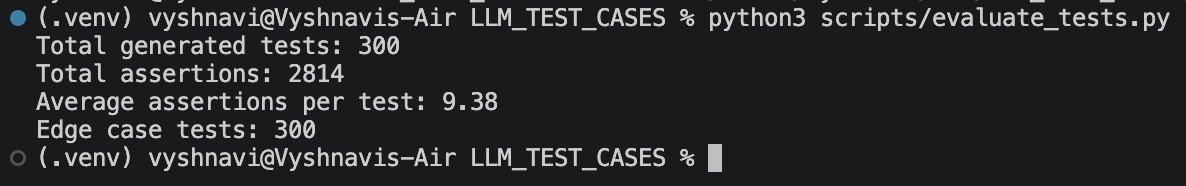
\includegraphics[width=0.85\linewidth]{Images/evaluate_tests.png}}
\caption{Evaluation results for the advanced prompting strategy showing 300 tests with 2814 total assertions}
\label{fig:evaluate_tests}
\end{figure}

Table~\ref{tab:failure_results} shows the failure analysis results.

\begin{table}[H]
\centering
\caption{Failure Analysis Results Advanced Prompt}
\label{tab:failure_results}
\begin{tabular}{lcc}
\toprule
\textbf{Category} & \textbf{Count} & \textbf{Percentage} \\
\midrule
Valid Python Code & 159 & 53\% \\
Syntax Errors & 141 & 47\% \\
No Assertions (after cleaning) & 215 & 72\% \\
Extra Text Issues & 88 & 29\% \\
\bottomrule
\end{tabular}
\end{table}

\begin{figure}[htbp]
\centerline{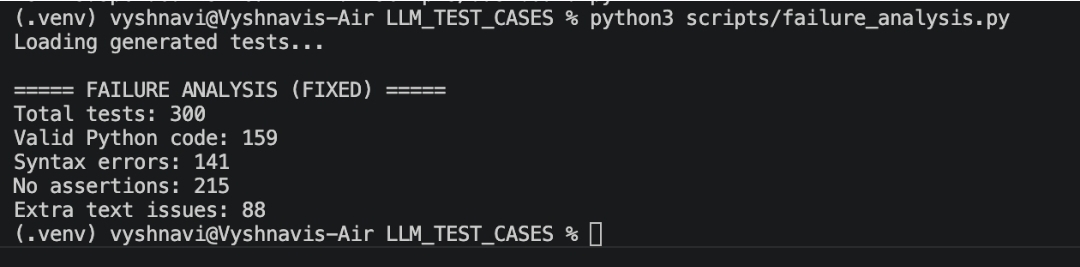
\includegraphics[width=0.85\linewidth]{Images/Failure_analysis.jpeg}}
\caption{Failure analysis output showing syntax validity and error breakdown across 300 generated tests}
\label{fig:Failure_analysis}
\end{figure}

Table~\ref{tab:prompt_comparison} provides a qualitative comparison across the three prompting strategies based on patterns observed across generated outputs during the experiments.

\begin{table}[H]
\centering
\caption{Qualitative Comparison of Prompting Strategies}
\label{tab:prompt_comparison}
\begin{tabular}{p{2.5cm}p{1.5cm}p{1.5cm}p{1.5cm}}
\toprule
\textbf{Attribute} & \textbf{Baseline} & \textbf{Context} & \textbf{Advanced} \\
\midrule
Assertion Count & Low & Moderate & High \\
Edge Cases & Rare & Some & Consistent \\
Code Structure & Minimal & Improved & Best \\
Extra Text & High & Moderate & Lower \\
Parameterization & None & None & Present \\
\bottomrule
\end{tabular}
\end{table}


\begin{figure}[htbp]
\centerline{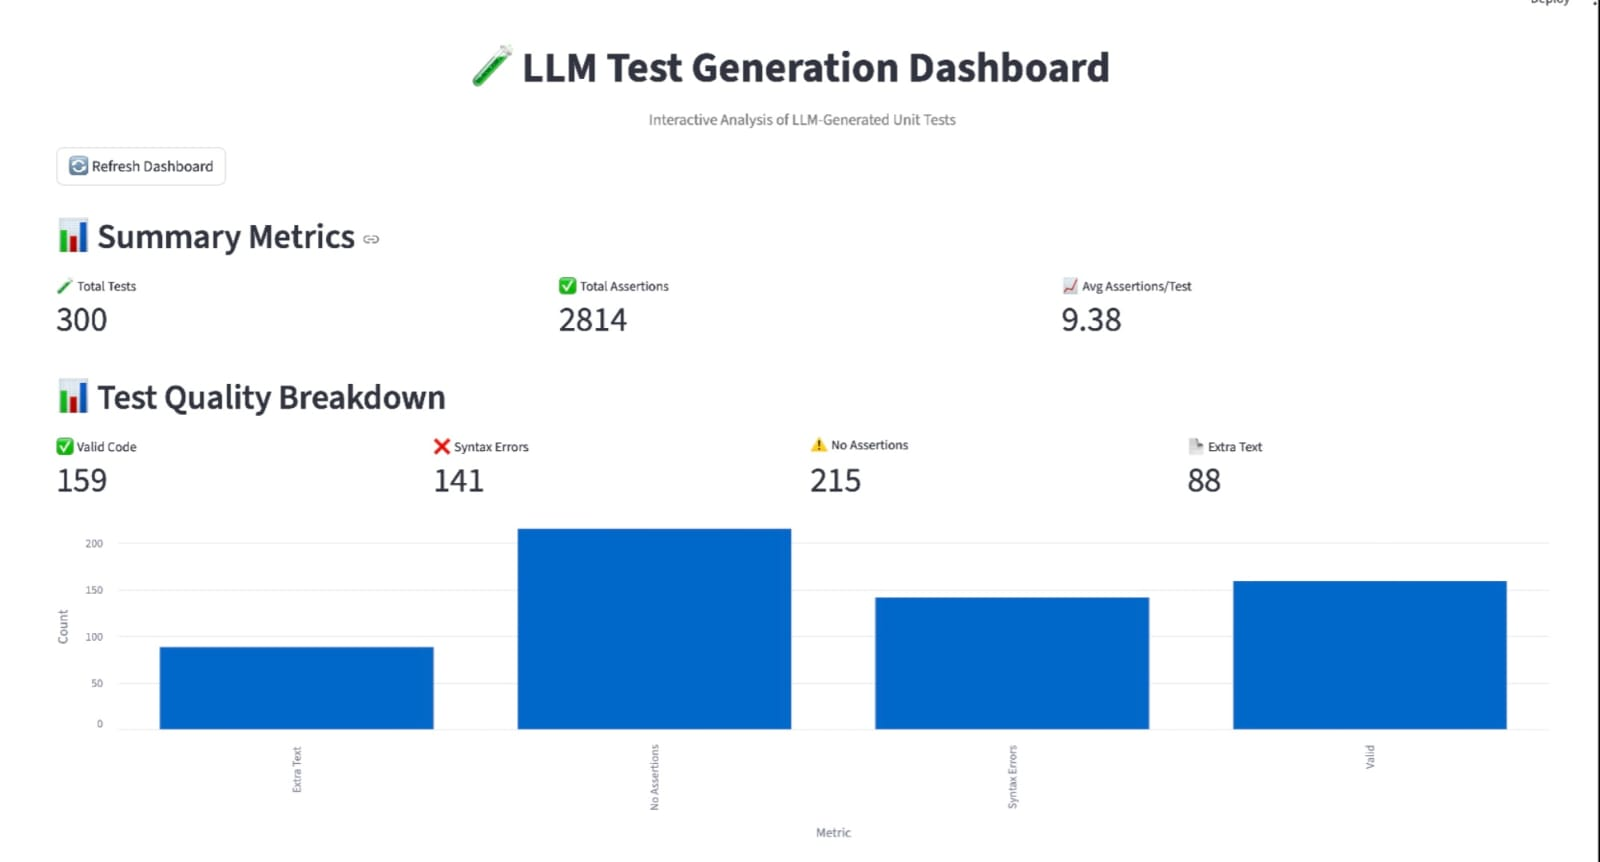
\includegraphics[width=0.85\linewidth]{Images/Dashboard.jpeg}}
\caption{Interactive Streamlit dashboard displaying test generation metrics and quality breakdown}
\label{fig:Dashboard}
\end{figure}

% ==================== 5. RESULTS ANALYSIS ====================
\section{Results Analysis}

\subsection{Interpretation of Findings}

The results show both strengths and limitations. The strengths are shown through the advanced prompt, which produced tests with an average of 9.38 assertions each. This is higher than what a developer would typically write in a quick unit test. Some form of edge-case content was detected in all generated tests, which indicates that the model is responsive to explicit instructions about boundary values and unusual inputs. A clear and consistent improvement in the output quality was shown through the progression from baseline context to advanced prompt. This suggests that prompt engineering is helpful with measurable impact and not just a theoretical idea.

The failure analysis reveals several limitations in a production setting. Python could not compile 47\% of the generated tests as they contained syntax errors. Despite being told to only produce code 29\% of the outputs included conversational text phrases like ``Here are the pytest unit tests'' or ``Note that the test assume\ldots''. The assertion-detection logic found that 215 out of 300 tests had no detectable assertions in the cleaned text. This reflects limitations in the detection method and indicates that the process could have removed valid assertion statements as well as extraneous text.

\subsection{Strengths}

\begin{itemize}[leftmargin=*]
    \item \textbf{High assertion density}: 9.38 assertions per test shows the model can generate detailed checks when prompted properly.
    \item \textbf{Complete edge-case coverage}: The advanced prompt achieved 100\% edge-case inclusion, which shows that explicit instructions help guide the model toward comprehensive testing.
    \item \textbf{Prompt sensitivity}: The importance of investing time in prompt design is supported by the improvement across prompting strategies.
    \item \textbf{Diverse test scenarios}: The model produced tests covering boundary values, normal inputs, and error conditions within a single response.
    \item \textbf{Scalability}: 
    Large numbers of tests can be efficiently generated and evaluated through the pipeline across multiple methods.
\end{itemize}

\subsection{Weaknesses}

\begin{itemize}[leftmargin=*]
    \item \textbf{Syntax reliability}: 47\% of the generated tests did not compile in Python indicating they are not immediately usable and need manual correction before being loaded by pytest.
    \item \textbf{Extra text in outputs}: 29\% (88 out of 300 generated tests) include conversational text. These would need to be filtered out before execution.
    \item \textbf{Missing assertions}: 215 out of 300 tests (72\%) had no detectable assertions after cleaning. These generated tests lacked meaningful validation so they would not effectively test the target function.
    \item \textbf{Fragility of the cleaning process}: When extraneous text is removed post-processing valid assertions may also be removed. This can contribute to the high number of tests with no detectable assertions after cleaning.
\end{itemize}

\subsection{Unexpected Outcomes}

Some of the unexpected outcomes from the results are as follows. First, we had anticipated that some sample methods would have names too generic for the edge-heuristic to produce useful suggestions and did not expect edge-case coverage to reach 100\%. The keyword-based detection turned out to be lenient enough that every test was flagged as containing edge-case content. Second, there was a disconnect between the raw assertion count (2814 across 300 tests) and the post-cleaning count. 215 tests had no detectable assertions after cleaning. This was unexpected and highlights a limitation in the cleaning pipeline rather than in the model's output. This emphasizes that evaluation tooling needs to be as carefully designed as the generation pipeline itself.

% ==================== 6. THREATS TO VALIDITY ====================
\section{Threats to Validity}

\subsection{Internal Validity}

The most significant internal threat is the limited sample of focal methods. They may not capture the full diversity of real-world code and individual outliers can skew the aggregate metrics substantially. It is difficult to ensure the results are representative due to a method with an unusually long or complex signature. This might produce very different results from a short utility function. Additionally, the results may not reflect what could be achieved with careful hyperparameter selection because we used the default Llama~3 parameters without tuning temperature. The non-deterministic nature of LLM inference also means that rerunning the experiment could produce somewhat different outputs.

\subsection{External Validity}

Our findings are based on a single model (Llama~3), a single programming language (Python), and a single testing framework (pytest). These results may not generalize to other programming environments. The pyMethods2Test dataset and different programming languages may produce different results. Despite being large and drawn from real projects they may not be representative of the full diversity of Python code in practice. Real-world systems may also involve complex interactions rather than the isolated function used in this study. 

\subsection{Construct Validity}

The metrics used rely on keyword matching, which is an approximate proxy for test quality. Assertion count and edge-case coverage may not fully capture all aspects of effective testing. Key-word heuristics may overestimate coverage since edge-case detection relies on it. Additionally, the cleaning process removed the extraneous text which may affect the detection of assertions. This can influence the reported results. As a result, the test quality should be interpreted as an approximation rather than an exact measure. 

% ==================== 7. CONCLUSION & FUTURE WORK ====================
\section{Conclusion and Future Work}

\subsection{Conclusion}

This project set out to answer two questions: Can a large language model generate useful unit tests for real-world Python functions, and does the way we ask it matter? The results suggest the answer to both questions is yes. Using Llama~3, we showed that well-structured prompts can produce tests with high assertion density and thorough edge-case coverage. Prompt engineering is one of the most effective tools as shown through the progression from our baseline prompt to the advanced prompt. It improves LLM output quality more effectively rather than simply switching to a larger model.

The results also show that LLM-generated tests are not ready to be used without human intervention. Text mixed with code, along with incorrect or missing assertions and syntax errors are common enough that a developer would need to review and edit every generated test before adding it to a test suite. Rather than full automation of test generation, the model provides a starting point that is faster to refine than writing from scratch.

\subsection{Future Work}

Several directions would strengthen and extend this work:

\begin{itemize}[leftmargin=*]
    \item \textbf{Execution-based evaluation}: Code coverage would provide a more meaningful picture of test quality than static analysis alone by running the generated tests with pytest and measuring actual pass/fail rates.
    \item \textbf{Larger sample sizes}: Scaling the experiment to hundreds or thousands of methods would produce statistically more robust results and allow for subgroup analysis by function complexity, project domain, and other factors.
    \item \textbf{Smarter output cleaning}: Replacing rule-based cleaning with an AST-aware parser that extracts Python code blocks from mixed text would significantly improve the usability of the generated output.
    \item \textbf{Model comparison}: To reveal how much of what we observed is specific to Llama~3 we can repeat the experiment with GPT-4, Claude, CodeLlama, and other models to see how much is a general characteristic of current LLMs.
    \item \textbf{Fine-tuning}: To improve quality and formatting consistency of generated tests we can train a model specifically on function test pairs from the pyMethods2Test dataset.
    \item \textbf{Interactive feedback loops}: Building a system where the model receives compilation errors from its own output and iterates on the fix could address the syntax-error problem without human involvement.
\end{itemize}

% ==================== REFERENCES ====================
\begin{thebibliography}{00}

\bibitem{tufano2022methods2test}
M.~Tufano, D.~Drain, A.~Svyatkovskiy, S.~K.~Deng, and N.~Sundaresan,
``Methods2Test: A dataset of focal methods mapped to test cases,''
in \textit{Proc. IEEE/ACM Int. Conf. Mining Software Repositories (MSR)},
2022, pp. 299--303.

\bibitem{pacheco2007randoop}
C.~Pacheco, S.~K.~Lahiri, M.~D.~Ernst, and T.~Ball,
``Feedback-directed random test generation,''
in \textit{Proc. Int. Conf. Software Engineering (ICSE)},
2007, pp. 75--84.

\bibitem{fraser2011evosuite}
G.~Fraser and A.~Arcuri,
``EvoSuite: Automatic test suite generation for object-oriented software,''
in \textit{Proc. ACM SIGSOFT Symp. Foundations of Software Engineering (FSE)},
2011, pp. 416--419.

\bibitem{chen2021codex}
M.~Chen, J.~Tworek, H.~Jun, Q.~Yuan, H.~P.~de~Oliveira~Pinto, J.~Kaplan, H.~Edwards, Y.~Burda, N.~Joseph, G.~Brockman, A.~Ray, R.~Puri, G.~Krueger, M.~Petrov, H.~Khlaaf, G.~Sastry, P.~Mishkin, B.~Chan, S.~Gray, N.~Ryder, M.~Pavlov, A.~Power, L.~Kaiser, M.~Bavarian, C.~Winter, P.~Tillet, F.~P.~Such, D.~Cummings, M.~Plappert, F.~Chanber, E.~Berner, C.~Lim, and W.~Zaremba,
``Evaluating large language models trained on code,''
\textit{arXiv preprint arXiv:2107.03374}, 2021.

\bibitem{touvron2023llama}
H.~Touvron, L.~Martin, K.~Stone, P.~Albert, A.~Almahairi, Y.~Babaei, N.~Bashlykov, S.~Batra, P.~Bhargava, S.~Bhosale, et~al.,
``Llama 2: Open foundation and fine-tuned chat models,''
\textit{arXiv preprint arXiv:2307.09288}, 2023.

\bibitem{li2023starcoder}
R.~Li, L.~B.~Allal, Y.~Zi, N.~Muennighoff, D.~Kocetkov, C.~Mou, M.~Marone, C.~Akiki, J.~Li, J.~Chim, et~al.,
``StarCoder: May the source be with you!''
\textit{arXiv preprint arXiv:2305.06161}, 2023.

\bibitem{wei2022chain}
J.~Wei, X.~Wang, D.~Schuurmans, M.~Bosma, B.~Ichter, F.~Xia, E.~Chi, Q.~Le, and D.~Zhou,
``Chain-of-thought prompting elicits reasoning in large language models,''
in \textit{Proc. Advances in Neural Information Processing Systems (NeurIPS)},
2022, pp. 24824--24837.

\bibitem{schafer2023adaptive}
M.~Sch{\"a}fer, S.~Nadi, A.~Eghbali, and F.~Tip,
``An empirical evaluation of using large language models for automated unit test generation,''
\textit{IEEE Trans. Software Engineering}, vol.~50, no.~1, pp.~85--105, 2024.

\bibitem{lemieux2023codamosa}
C.~Lemieux, J.~P.~Inala, S.~K.~Lahiri, and S.~Sen,
``CodaMosa: Escaping coverage plateaus in test generation with pre-trained large language models,''
in \textit{Proc. Int. Conf. Software Engineering (ICSE)},
2023, pp. 919--931.

\bibitem{yuan2023chatgpt}
Z.~Yuan, Y.~Lou, M.~Liu, S.~Ding, K.~Wang, Y.~Chen, and X.~Peng,
``No more manual tests? Evaluating and improving ChatGPT for unit test generation,''
\textit{arXiv preprint arXiv:2305.04207}, 2023.

\end{thebibliography}

\end{document}
